\documentclass[tikz,border=8pt]{standalone}
% Shared look for every TikZ diagram. Load with % Shared look for every TikZ diagram. Load with % Shared look for every TikZ diagram. Load with \input{../../tools/tikz-style.tex}
\usepackage[T1]{fontenc}
\usepackage{lmodern}
\renewcommand{\sfdefault}{lmr}  % diagrams use the same serif as the text
\usetikzlibrary{arrows.meta, positioning, shapes.geometric, calc, fit, backgrounds}
\definecolor{cblue}{HTML}{4C78A8}
\definecolor{corange}{HTML}{F58518}
\definecolor{cgreen}{HTML}{54A24B}
\definecolor{cred}{HTML}{E45756}
\definecolor{cpurple}{HTML}{B279A2}
\definecolor{cgrey}{HTML}{6B6B6B}
\tikzset{
  every picture/.style={font=\sffamily, line width=1.2pt},
  box/.style={draw=#1, fill=#1!12, rounded corners=4pt, align=center, inner sep=7pt, minimum height=1.1cm},
  box/.default=cgrey,
  arrow/.style={-{Stealth[length=3mm]}, draw=cgrey, line width=1.4pt},
  title/.style={font=\sffamily\bfseries\Large},
  note/.style={font=\sffamily\small, text=cgrey, align=center},
}
\AtBeginDocument{\hyphenpenalty=10000 \exhyphenpenalty=10000}

\usepackage[T1]{fontenc}
\usepackage{lmodern}
\renewcommand{\sfdefault}{lmr}  % diagrams use the same serif as the text
\usetikzlibrary{arrows.meta, positioning, shapes.geometric, calc, fit, backgrounds}
\definecolor{cblue}{HTML}{4C78A8}
\definecolor{corange}{HTML}{F58518}
\definecolor{cgreen}{HTML}{54A24B}
\definecolor{cred}{HTML}{E45756}
\definecolor{cpurple}{HTML}{B279A2}
\definecolor{cgrey}{HTML}{6B6B6B}
\tikzset{
  every picture/.style={font=\sffamily, line width=1.2pt},
  box/.style={draw=#1, fill=#1!12, rounded corners=4pt, align=center, inner sep=7pt, minimum height=1.1cm},
  box/.default=cgrey,
  arrow/.style={-{Stealth[length=3mm]}, draw=cgrey, line width=1.4pt},
  title/.style={font=\sffamily\bfseries\Large},
  note/.style={font=\sffamily\small, text=cgrey, align=center},
}
\AtBeginDocument{\hyphenpenalty=10000 \exhyphenpenalty=10000}

\usepackage[T1]{fontenc}
\usepackage{lmodern}
\renewcommand{\sfdefault}{lmr}  % diagrams use the same serif as the text
\usetikzlibrary{arrows.meta, positioning, shapes.geometric, calc, fit, backgrounds}
\definecolor{cblue}{HTML}{4C78A8}
\definecolor{corange}{HTML}{F58518}
\definecolor{cgreen}{HTML}{54A24B}
\definecolor{cred}{HTML}{E45756}
\definecolor{cpurple}{HTML}{B279A2}
\definecolor{cgrey}{HTML}{6B6B6B}
\tikzset{
  every picture/.style={font=\sffamily, line width=1.2pt},
  box/.style={draw=#1, fill=#1!12, rounded corners=4pt, align=center, inner sep=7pt, minimum height=1.1cm},
  box/.default=cgrey,
  arrow/.style={-{Stealth[length=3mm]}, draw=cgrey, line width=1.4pt},
  title/.style={font=\sffamily\bfseries\Large},
  note/.style={font=\sffamily\small, text=cgrey, align=center},
}
\AtBeginDocument{\hyphenpenalty=10000 \exhyphenpenalty=10000}

\begin{document}
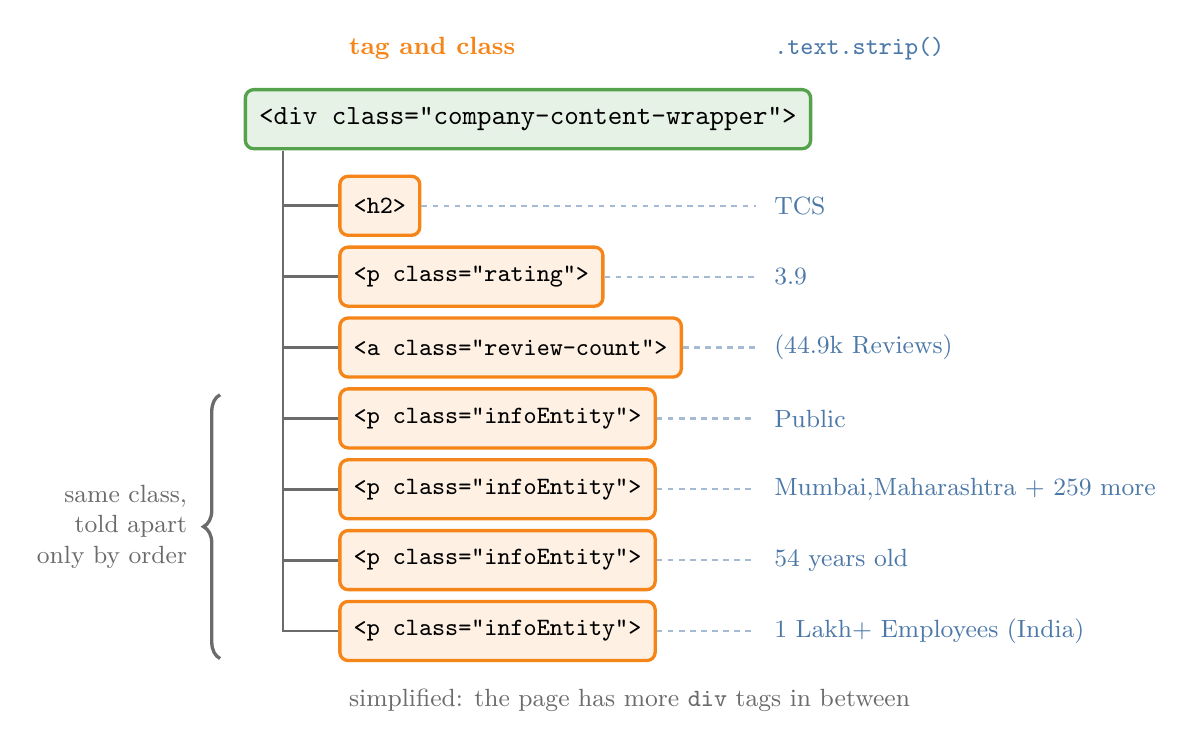
\begin{tikzpicture}[
    tg/.style={draw=corange, fill=corange!12, rounded corners=3pt, font=\small\ttfamily, inner sep=5pt, anchor=west, minimum height=0.75cm},
    val/.style={font=\small, anchor=west, text=cblue},
    edge/.style={draw=cgrey, line width=1pt}]
  % root: the container for one company
  \node[tg, draw=cgreen, fill=cgreen!14, font=\ttfamily\bfseries] (root) at (0,0) {<div class="company-content-wrapper">};
  \def\x{1.2}
  \foreach \y/\t/\v [count=\i] in {
      -1.1/{<h2>}/{TCS},
      -2.0/{<p class="rating">}/{3.9},
      -2.9/{<a class="review-count">}/{(44.9k Reviews)},
      -3.8/{<p class="infoEntity">}/{Public},
      -4.7/{<p class="infoEntity">}/{Mumbai,Maharashtra + 259 more},
      -5.6/{<p class="infoEntity">}/{54 years old},
      -6.5/{<p class="infoEntity">}/{1 Lakh+ Employees (India)}} {
    \node[tg] (n\i) at (\x,\y) {\t};
    \draw[edge] (0.5,-0.4) |- (n\i.west);
    \node[val] at (6.6,\y) {\v};
    \draw[draw=cblue!50, line width=0.8pt, dash pattern=on 2pt off 2pt] (n\i.east) -- (6.5,\y);
  }
  \node[font=\bfseries\small, text=corange, anchor=west] at (1.2,0.9) {tag and class};
  \node[font=\bfseries\small, text=cblue, anchor=west] at (6.6,0.9) {\texttt{.text.strip()}};
  \node[note, anchor=north west] at (1.2,-7.1) {simplified: the page has more \texttt{div} tags in between};
  \draw[decorate, decoration={brace, amplitude=6pt, mirror}, draw=cgrey] (-0.3,-3.5) -- (-0.3,-6.85)
    node[midway, left=8pt, note, align=right] {same class,\\told apart\\only by order};
\end{tikzpicture}
\end{document}
